\subsection{Log Figures}
\label{App:LogFigures}
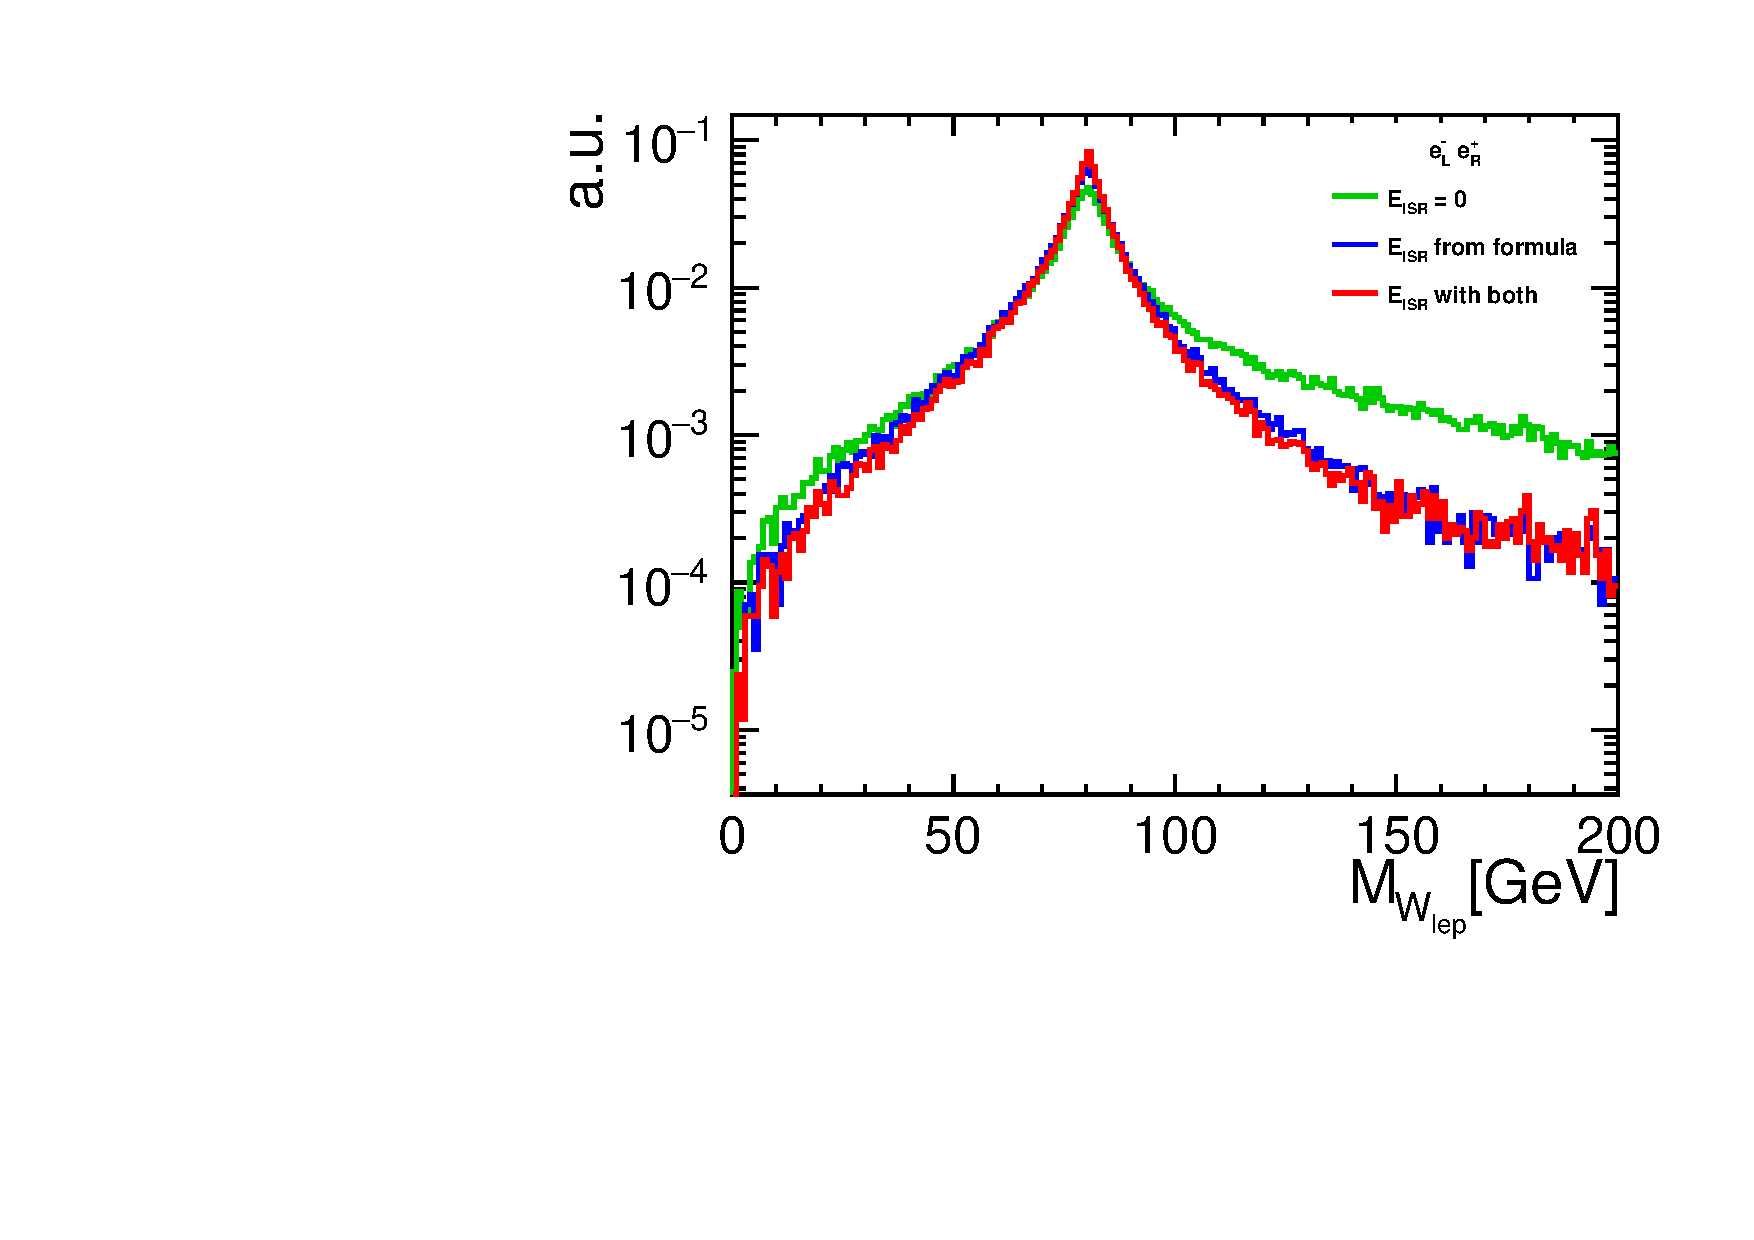
\includegraphics[width=0.49\textwidth]{\imagepath/Mass3_log.pdf}
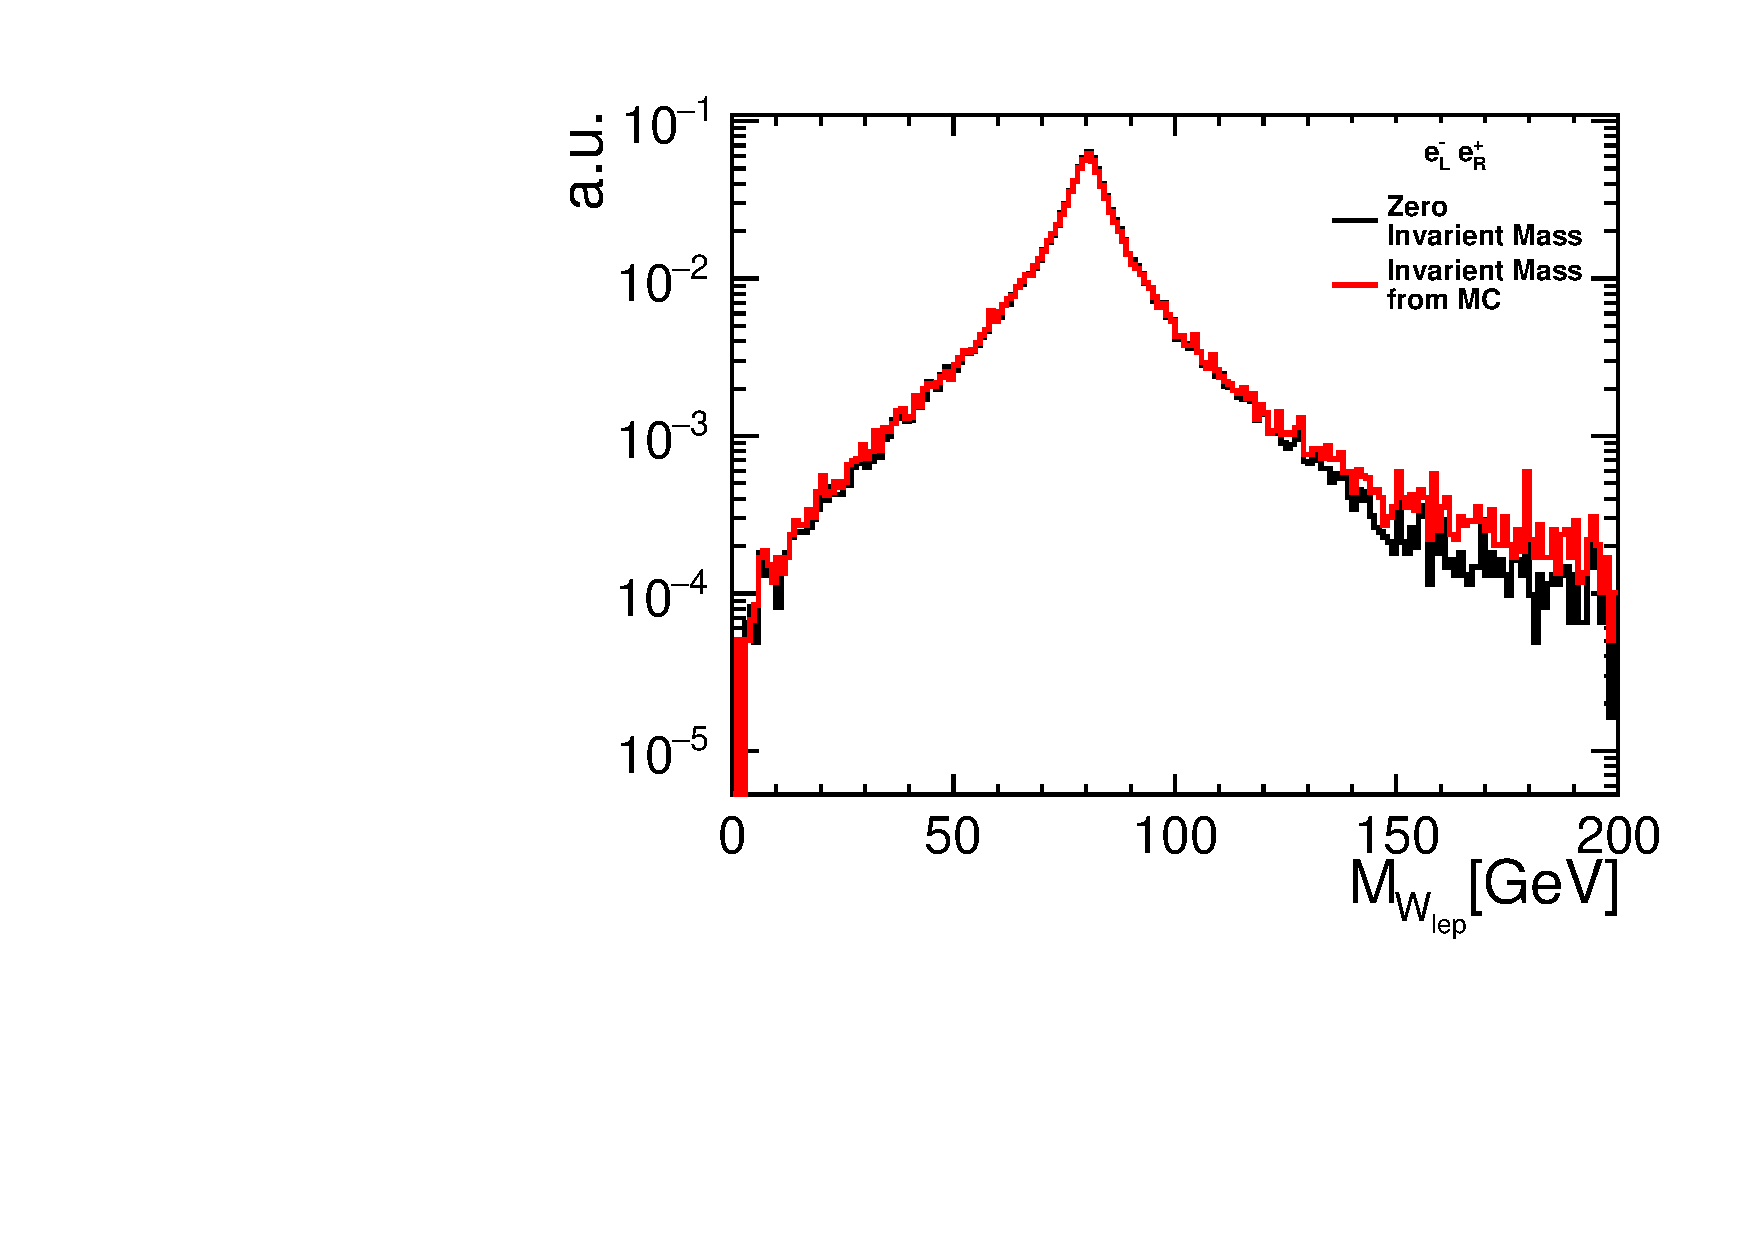
\includegraphics[width=0.49\textwidth]{\imagepath/Mass_log.pdf}

\subsection{Steering file}
\label{App:SteeringFile}

The layout of the steering file:

\begin{itemize}
	\item IsolatedLeptonTaggingProcessor
		\begin{itemize}
			\item InputCollection: PandoraPFOs
			\item Electron Weight:\\
            \texttt{$/cvmfs/ilc.desy.de/sw/x86\_64\_gcc49\_sl6/v02-00-02/MarlinReco/v01-25/Analysis/$}
            \texttt{$IsolatedLeptonTagging/weights/yyxyev\_yyxyyx\_500.mILD\_l5\_o1\_v02$}
			\item Muon Weight: \\
            \texttt{$/cvmfs/ilc.desy.de/sw/x86\_64\_gcc49\_sl6/v02-00-02/MarlinReco/v01-25/Analysis/$}
            \texttt{$IsolatedLeptonTagging/weights/yyxylv\_yyxyyx\_woYoke\_500.mILD\_l5\_o1\_v02$}
			\item OutputCollection: Isoleps
			\item OutputCollection: PFOsWithoutIsoleps
		\end{itemize}
	\item FastJetProcessor (Beam Background Removal)
		\begin{itemize}
			\item InputCollection: PFOsWithoutIsoleps
			\item OutputCollection: PFOsOverlayRemoved
		\end{itemize}
	\item FastJetProcessor (Jet Clustering)
		\begin{itemize}
			\item InputCollection: PFOsOverlayRemoved
			\item OutputCollection: FastJets
			\item OutputCollection: PFOsFromFastJet
		\end{itemize}
	\item MyFirstObservableProcessor
		\begin{itemize}
			\item InputCollection: MCParticle
			\item InputCollection: PFOsOverlayRemoved
			\item InputCollection: Isoleps
			\item InputCollection: FastJets
		\end{itemize}
\end{itemize}
with LCIO input files:\\
\texttt{$/pnfs/desy.de/ilc/prod/ilc/mc-opt-3/ild/dst-merged/500-TDR\_ws/4f\_WW\_semileptonic/$}
\texttt{$ILD\_l5\_o1\_v02/v02-00-01/rv02-00-01.sv02-00-01.mILD\_l5\_o1\_v02.E500-TDR\_ws.I250018.$}
\texttt{$P4f\_ww\_sl.eL.pR.n0*.d\_dstm\_10318\_*.slcio$}.
\\\\
The only deviation from this format of steering file was when the beam background removal was cheated. Here the "FastJetProcessor (Beam Background Removal)" processor was replaced with a "TrueJet" processor with MCParticle input collection followed by a "TJJetRecoParticleFinder" processor which outputs a collection RecosFromHadronicJets. This RecosFromHadronicJets collection was then used as the input to the "FastJetProcessor (Jet Clustering)" processor.

\begin{itemize}
	\item IsolatedLeptonTaggingProcessor
		\begin{itemize}
			\item InputCollection: PandoraPFOs
			\item Electron Weight:\\
            \texttt{$/cvmfs/ilc.desy.de/sw/x86\_64\_gcc49\_sl6/v02-00-02/MarlinReco/v01-25/Analysis/$}
            \texttt{$IsolatedLeptonTagging/weights/yyxyev\_yyxyyx\_500.mILD\_l5\_o1\_v02$}
			\item Muon Weight: \\
            \texttt{$/cvmfs/ilc.desy.de/sw/x86\_64\_gcc49\_sl6/v02-00-02/MarlinReco/v01-25/Analysis/$}
            \texttt{$IsolatedLeptonTagging/weights/yyxylv\_yyxyyx\_woYoke\_500.mILD\_l5\_o1\_v02$}
			\item OutputCollection: Isoleps
			\item OutputCollection: PFOsWithoutIsoleps
		\end{itemize}
	\item TrueJet
		\begin{itemize}
			\item InputCollection: MCParticle
        \end{itemize}
    \item TJJetRecoParticleFinder
        \begin{itemize}
			\item OutputCollection: RecosFromHadronicJets
		\end{itemize}
	\item FastJetProcessor (Jet Clustering)
		\begin{itemize}
			\item InputCollection: RecosFromHadronicJets
			\item OutputCollection: FastJets
			\item OutputCollection: PFOsFromFastJet
		\end{itemize}
	\item MyFirstObservableProcessor
		\begin{itemize}
			\item InputCollection: MCParticle
			\item InputCollection: PFOsOverlayRemoved
			\item InputCollection: Isoleps
			\item InputCollection: FastJets
		\end{itemize}
\end{itemize}


\subsection{Derivation of the ISR energy ${E}_{\gamma}$ with non-trivial ${m}_{\gamma}$ and ${m}_{\nu}$}
\label{App:Derivation}

Our initial assumptions are that the system is in the center of mass frame with an invariant mass of 500 GeV. The system contains a visible 4-momentum ${p}^{\mu} = ( E,  {p}_{x}, {p}_{y}, {p}_{z})$ and an invisible 4-momentum (a neutrino ${p}^{\mu}_{\nu} = ( {E}_{\nu},  {p}_{\nu,x}, {p}_{\nu,y}, {p}_{\nu,z})$ and an ISR photon $ {p}^{\mu}_{\gamma} = ( {E}_{\gamma}, 0, 0,  {p}_{\gamma}) )$. Both the neutrino and the photon have a non trivial invariant mass leading to the following equations.\\\\
Conservation of 3-momentum
\begin{align}
{p}_{x} + {p}_{\nu,x}&=0\\
{p}_{y} + {p}_{\nu,y}&=0\\
{p}_{z} + {p}_{\nu,z} + {p}_{\gamma} &= 0\\
 \end{align}
Conservation of Energy
 \begin{align}
E + {E}_{\nu} + {E}_{\gamma} &= 500
 \end{align}
Energy-Momentum equations
 \begin{align}
{E}_{\nu}^{2} &= {p}_{\nu}^{2} +{m}_{\nu}^{2}\\
{E}_{\gamma}^{2} &= {p}_{\gamma}^{2} +{m}_{\gamma}^{2}\\
 \end{align}
For a unique solution of ${E}_{\gamma}$ we require 2 more constraints on ${m}_{\gamma}$ and ${m}_{\nu}$ which have yet to be imposed, but assuming these constraints are independent of ${E}_{\gamma}$ we can arrive at a solution as follows.\\

From conservation of 3-momentum
 \begin{align}
 {p}_{\nu}^{2} &= {p}_{\nu,x}^{2} + {p}_{\nu,y}^{2} + {p}_{\nu,z}^{2} \\
 					&= {p}_{x}^{2} + {p}_{y}^{2} + {({p}_{\gamma} + {p}_{z})}^{2} \\
 					&= {p}^{2} + {p}_{\gamma}^{2} + 2{p}_{\gamma}{p}_{z} \\
 					&=  {p}^{2} + {E}_{\gamma}^{2} - {m}_{\gamma}^{2} + 2{p}_{\gamma}{p}_{z} \, .
 \end{align}
Conservation of energy then gives us,
 \begin{align}
 {(500 - E)}^2 - {p}^{2} &= {({E}_{\nu} + {E}_{\gamma})}^2  - {p}^{2} \\
 								   &= {E}_{\nu}^{2}  + {E}_{\gamma}^{2} - {p}^{2} + 2{E}_{\gamma}{E}_{\nu}\\
 								   &= {p}_{\nu}^{2}  + {m}_{\nu}^{2} + {E}_{\gamma}^{2} - {p}^{2} + 2{E}_{\gamma}{E}_{\nu}\, .
 \end{align}
Substituting in the expression for ${p}_{\nu}$,
 \begin{align}
{(500 - E)}^2 - {p}^{2} &=  \Cancel[red]{{p}^{2}} + {E}_{\gamma}^{2} - {m}_{\gamma}^{2} + 2{p}_{\gamma}{p}_{z} + {m}_{\nu}^{2} + {E}_{\gamma}^{2} - \Cancel[red]{{p}^{2}} + 2{E}_{\gamma}{E}_{\nu}\\
  {(500 - E)}^2 - {p}^{2} + {m}_{\gamma}^{2} - {m}_{\nu}^{2}
  								&=  2({E}_{\gamma}^{2} + {p}_{\gamma}{p}_{z} + {E}_{\gamma}{E}_{\nu})\\
  								&=  2( \Cancel[red]{{E}_{\gamma}^{2}} + {p}_{\gamma}{p}_{z} + {E}_{\gamma}[500 -  \Cancel[red]{{E}_{\gamma}} - E])\\
  								&=  2( {p}_{\gamma}{p}_{z} + 500{E}_{\gamma} - E{E}_{\gamma} )\, .
 \end{align}
 Where we have one again used conservation of energy.\\\\
 For convenience lets define
\begin{equation}
    {\lambda} = \frac{1}{2}[{(500 - E)}^2 - {p}^{2} + {m}_{\gamma}^{2} - {m}_{\nu}^{2}]
\end{equation}

 and use  ${E}_{\gamma}^{2} = {p}_{\gamma}^{2} +{m}_{\gamma}^{2} $ to arrive at a solvable equation in ${E}_{\gamma} $\, .
  \begin{align}
 {\lambda} &=   {p}_{\gamma}{p}_{z} + 500{E}_{\gamma} - E{E}_{\gamma} \\
  [{\lambda} - (500 - E){E}_{\gamma} ] &=   {p}_{\gamma}{p}_{z} \\
    {[{\lambda} - (500 - E){E}_{\gamma} ]}^{2} &= ({E}_{\gamma}^{2} - {m}_{\gamma}^{2}){p}_{z}^{2} \\
    {\lambda}^{2} - 2{\lambda}(500 - E){E}_{\gamma}  + {(500 - E)}^{2}{{E}_{\gamma}}^{2} &=   {p}_{z}^{2}{E}_{\gamma}^{2} - {p}_{z}^{2}{m}_{\gamma}^{2} \\
        [{(500 - E)}^{2} -   {p}_{z}^{2}]{E}_{\gamma}^{2}  - 2{\lambda}(500 - E){E}_{\gamma} +  ({\lambda}^{2} + {p}_{z}^{2}{m}_{\gamma}^{2})  &= 0
     \end{align}
This can be solved with the quadratic formula to give,
  \begin{align}
 {E}_{\gamma} &= \frac{{\lambda}(500 - E)  \pm \sqrt{ {\lambda}^{2}{(500 - E)}^{2} - [{(500 - E)}^{2} -   {p}_{z}^{2}][{\lambda}^{2} + {p}_{z}^{2}{m}_{\gamma}^{2}] }}{{(500 - E)}^{2} -   {p}_{z}^{2}}\\
 					&= \frac{{\lambda}(500 - E)  \pm {p}_{z}\sqrt{ {\lambda}^{2} - [{(500 - E)}^{2} -   {p}_{z}^{2}]{m}_{\gamma}^{2}}}{{(500 - E)}^{2} -   {p}_{z}^{2}}\, .
     \end{align}
As expected, the solution with ${m}_{\gamma} = {m}_{\nu} =0$  reduces to the previously calculated solution
\begin{align}
 {\lambda} &= \frac{1}{2}[{(500 - E)}^2 - {p}^{2} + \cancelto{0}{{m}_{\gamma}^{2} }- \cancelto{0}{{m}_{\nu}^{2}}]\\
  {E}_{\gamma} &= \frac{{\lambda}(500 - E)  \pm {p}_{z}\sqrt{ {\lambda}^{2} - [{(500 - E)}^{2} -   {p}_{z}^{2}] \cancelto{0}{{m}_{\gamma}^{2}}}}{{(500 - E)}^{2} -   {p}_{z}^{2}}\\
  &= \frac{{\lambda}[(500 - E)  \pm {p}_{z}]}{{(500 - E)}^{2} -   {p}_{z}^{2}} \\
  &= \frac{ \frac{1}{2}[{(500 - E)}^2 - {p}^{2}]}{(500 - E)  \mp {p}_{z}} \\
   &= \frac{ {(500 - E)}^2 - {p}^{2}}{1000 -2 E  \mp 2{p}_{z}}\, .
     \end{align}
  c.f Ivan's result \cite{IvanMarchesini}
  \\
It can also easily be shown for this case that the two solutions correspond to ISR photons travelling parallel or anti-parallel to the z axis. The $\mp$ in the denominator hence corresponds to the sign of the photons z momentum,

\begin{equation}
  {E}_{\gamma} = \frac{ {(500 - E)}^2 - {p}^{2}}{1000 -2 E + 2sgn({p}_{\gamma}) {p}_{z}}
     \end{equation}
\begin{equation}
 {E}_{\gamma} = \frac{{\lambda}(500 - E) + sgn({p}_{\gamma}) {p}_{z}\sqrt{ {\lambda}^{2} - [{(500 - E)}^{2} -   {p}_{z}^{2}]{m}_{\gamma}^{2}}}{{(500 - E)}^{2} -   {p}_{z}^{2}}\, .
     \end{equation}
